% !TEX TS-program = knitr
\documentclass[handout]{beamer}
\setbeamercovered{dynamic}

\usetheme{Marburg}
\setbeamertemplate{navigation symbols}{} 
\setbeamertemplate{footline}
{
  \leavevmode%
  \hbox{%
  \begin{beamercolorbox}[wd=.333333\paperwidth,ht=2.25ex,dp=1ex,center]{author in head/foot}%
    \usebeamerfont{author in head/foot} $\ $ \insertshortauthor%~~\beamer@ifempty{\insertshortinstitute}{}{(\insertshortinstitute)}
  \end{beamercolorbox}%
  \begin{beamercolorbox}[wd=.333333\paperwidth,ht=2.25ex,dp=1ex,center]{title in head/foot}%
    \usebeamerfont{title in head/foot} \insertinstitute
  \end{beamercolorbox}%
  \begin{beamercolorbox}[wd=.333333\paperwidth,ht=2.25ex,dp=1ex,right]{date in head/foot}%
    \usebeamerfont{date in head/foot}\insertshortdate{}\hspace*{2em}
    \insertframenumber{} / \inserttotalframenumber\hspace*{2ex} 
  \end{beamercolorbox}}%
  \vskip0pt%
}

\usepackage{amsmath}
\usepackage{caption}
\usepackage{color}
\usepackage{enumerate}
\usepackage{listings}
\usepackage{hyperref}
\usepackage{mathrsfs}
\usepackage{natbib}
\usepackage{url}

\providecommand{\all}{\ \forall \ }
\providecommand{\bs}{\backslash}
\providecommand{\e}{\varepsilon}
\providecommand{\E}{\ \exists \ }
\providecommand{\lm}[2]{\lim_{#1 \rightarrow #2}}
\providecommand{\m}[1]{\mathbb{#1}}
\providecommand{\nv}{{}^{-1}}
\providecommand{\ov}[1]{\overline{#1}}
\providecommand{\p}{\newpage}
\providecommand{\q}{$\quad$ \newline}
\providecommand{\rt}{\rightarrow}
\providecommand{\Rt}{\Rightarrow}
\providecommand{\vc}[1]{\boldsymbol{#1}}
\providecommand{\wh}[1]{\widehat{#1}}

\hypersetup{colorlinks,linkcolor=,urlcolor=blue}
\numberwithin{equation}{section}

\definecolor{dkgreen}{rgb}{0,0.6,0}
\definecolor{gray}{rgb}{0.5,0.5,0.5}
\definecolor{mauve}{rgb}{0.58,0,0.82}

\lstset{ 
  language=C,                % the language of the code
  basicstyle= \footnotesize,           % the size of the fonts that are used for the code
  numberstyle= \tiny \color{white},  % the style that is used for the line-numbers
  stepnumber=2,                   % the step between two line-numbers. 
  numbersep=5pt,                  % how far the line-numbers are from the code
  backgroundcolor=\color{white},      % choose the background color. You must add \usepackage{color}
  showspaces=false,               % show spaces adding particular underscores
  showstringspaces=false,         % underline spaces within strings
  showtabs=false,                 % show tabs within strings adding particular underscores
  frame=lrb,                   % adds a frame around the code
  rulecolor=\color{black},        % if not set, the frame-color may be changed on line-breaks within not-black text 
  tabsize=2,                      % sets default tabsize to 2 spaces
  captionpos=t,                   % sets the caption-position 
  breaklines=true,                % sets automatic line breaking
  breakatwhitespace=false,        % sets if automatic breaks should only happen at whitespace
  %title=\lstname,                   % show the filename of files included with \lstinputlisting;
  keywordstyle=\color{blue},          % keyword style
  commentstyle=\color{gray},       % comment style
  stringstyle=\color{dkgreen},         % string literal style
  escapeinside={\%*}{*)},            % if you want to add LaTeX within your code
  morekeywords={*, ...},               % if you want to add more keywords to the set
  xleftmargin=0.053in, % left horizontal offset of caption box
  xrightmargin=-.03in % right horizontal offset of caption box
}

%\DeclareCaptionFont{white}{\color{white}}
%\DeclareCaptionFormat{listing}{\parbox{\textwidth}{\colorbox{gray}{\parbox{\textwidth}{#1#2#3}}\vskip-0.05in}}
%\captionsetup[lstlisting]{format = listing, labelfont = white, textfont = white}
%For caption-free listings, comment out the 3 lines above and uncomment the 2 lines below.
 \captionsetup{labelformat = empty, labelsep = none}
 \lstset{frame = single}


\title{Describing Relationships \emph{Among} Variables (Ch. 4)}
\author{Yifan Zhu}
\date{}
\institute{Iowa State University}

\usepackage{Sweave}
\begin{document}
\Sconcordance{concordance:ch4part2.tex:ch4part2.Rnw:%
1 87 1 1 7 6 1 1 0 266 1}


\begin{frame}
\titlepage
 \end{frame}
 
 \AtBeginSection[]
{
   \begin{frame}
       \frametitle{Outline}
       \tableofcontents[currentsection]
   \end{frame}
}

\section{Polynomial Regression}

\begin{frame}
\frametitle{Polynomial Regression}
\begin{itemize}
\pause \item Simple linear regression: fit a line:
\begin{align*}
y_i \approx b_0 + b_1 x_i
\end{align*}
\pause \item Polynomial regression: fit a polynomial:
\begin{align*}
y_i \approx b_0 + b_1 x_i + b_2 x_i^2 + b_3 x_i ^3 + \cdots + b_{p-1} x_i^{p-1}
\end{align*}
\begin{itemize}
\pause \item The $p$ coefficients $b_0, b_1, \ldots, b_{p-1}$ are estimated by minimizing the loss function below using the least squares principle:
\pause \begin{align*}
S(b_0, \ldots, b_{p-1}) = \sum_{i = 1}^n (y_i -  (b_0 + b_1 x_i  + \cdots + b_{p-1} x_i^{p-1}))^2
\end{align*}
\pause \item In practice, we make a computer find the coefficients for us. This class uses JMP. See \url{https://www.stat.iastate.edu/statistical-software-jmp} for JMP installation and JMP Help and Resource.
\end{itemize}
\end{itemize}
\end{frame}




\begin{frame}
\frametitle{Example: fly ash cylinders}
\begin{itemize}
\pause \item A researcher studied the compressive strength of concrete-like fly ash cylinders. The cylinders were made with varying amounts of ammonium phosphate as an additive.
\pause \item We want to investigate the relationship between the amount ammonium phosphate added and compressive strength.
\end{itemize}

\begin{center}
\setkeys{Gin}{width=.75\textwidth} \includegraphics<3->{../../fig/flyashdata.png}
\end{center}
\end{frame}




\begin{frame}
\frametitle{Simple linear regression fit: $\wh{y}_i = 1498.4 - .6381x_i$}
\begin{center}
\setkeys{Gin}{width=.75\textwidth} 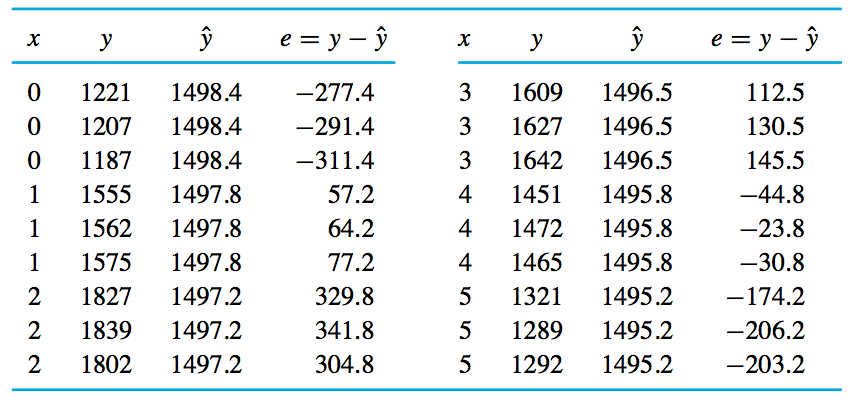
\includegraphics{../../fig/flyashdataresid.png}
\end{center}
\begin{minipage}[b]{.48\linewidth}
\setkeys{Gin}{width=.75\textwidth} 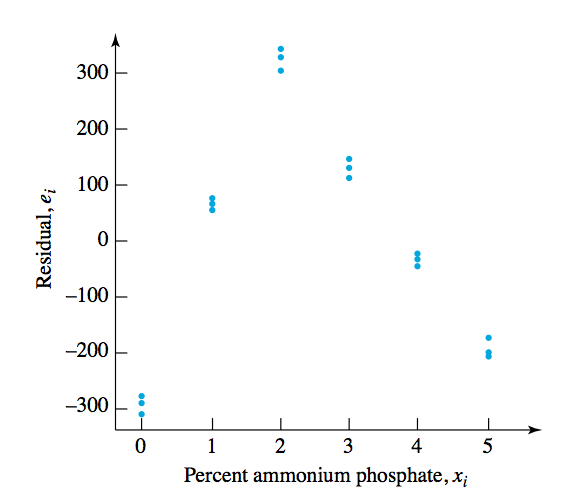
\includegraphics{../../fig/flyashslrfit.png}
\end{minipage}
\begin{minipage}[b]{.48\linewidth}
\setkeys{Gin}{width=.75\textwidth} 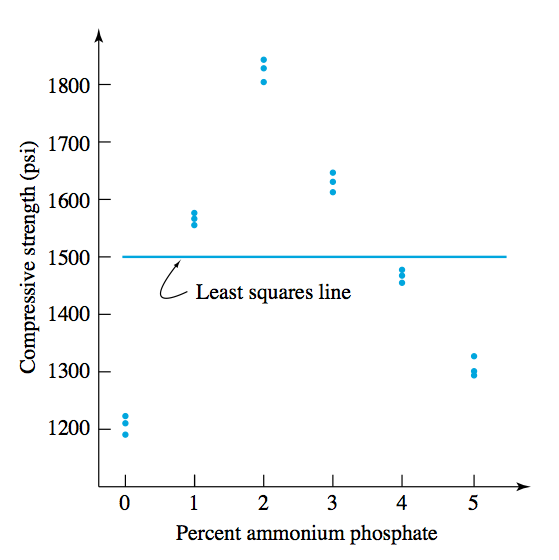
\includegraphics{../../fig/flyashslrfit2.png}
\end{minipage}
\end{frame}

\begin{frame}
\frametitle{Quadratic fit: $\wh{y}_i = 1242.9 + 382.7x - 76.7x_i^2$}
\setkeys{Gin}{width=1\textwidth} 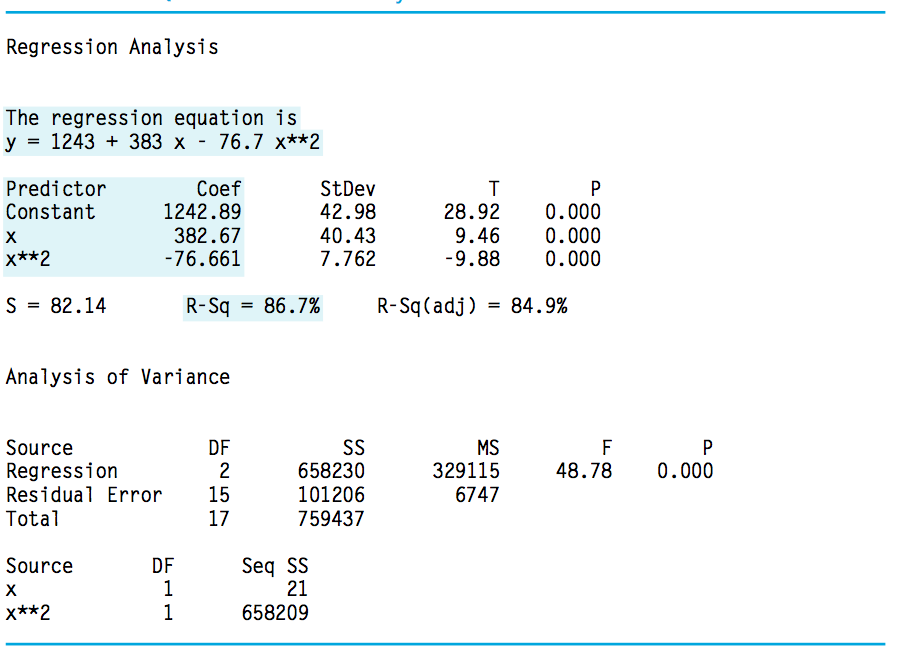
\includegraphics{../../fig/flyashquadfitoutput.png}
\end{frame}

\begin{frame}
\frametitle{Quadratic fit: $\wh{y}_i = 1242.9 + 382.7x - 76.7x_i^2$}
\setkeys{Gin}{width=.9\textwidth} 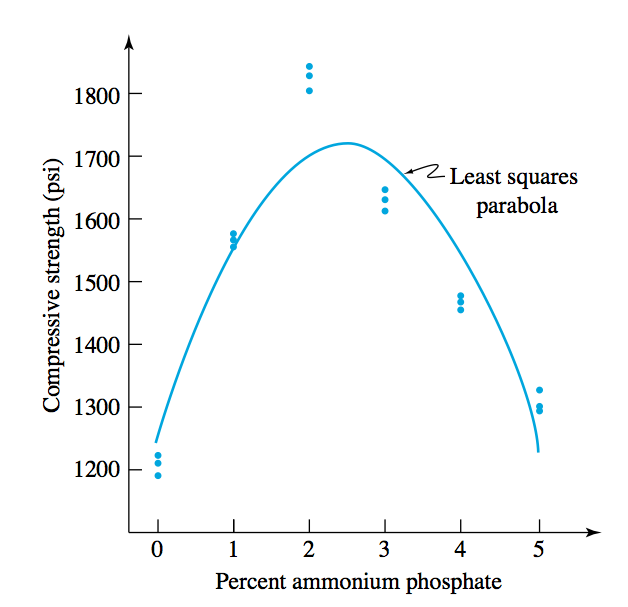
\includegraphics{../../fig/flyashquadfitfit.png}
\end{frame}

\begin{frame}
\frametitle{$R^2 = 86.7\%$}
\begin{itemize}
\pause \item The parabolic fit explained 86.7\% of the variation in compressive strength. 
\pause \item Note: for polynomial regression (and later, multiple regression) $R^2$ does not equal the squared correlation $r_{xy}^2$ between $x$ and $y$. 
\pause \item Instead, $R^2 = r_{y \wh{y}}^2$: 
\pause \begin{align*}
 r_{y \wh{y}} = \frac{\sum(y_i - \ov{y})(\wh{y}_i - \ov{\wh{y}}_i)}{\sqrt{\sum (y_i - \ov{y})^2}\sqrt{\sum (\wh{y}_i - \ov{\wh{y}}_i)^2}}
\end{align*}
\end{itemize}
\end{frame}

\begin{frame}
\frametitle{\small Residuals for the quadratic fit have less of a pattern than those of the linear fit.}
\setkeys{Gin}{width=.9\textwidth} 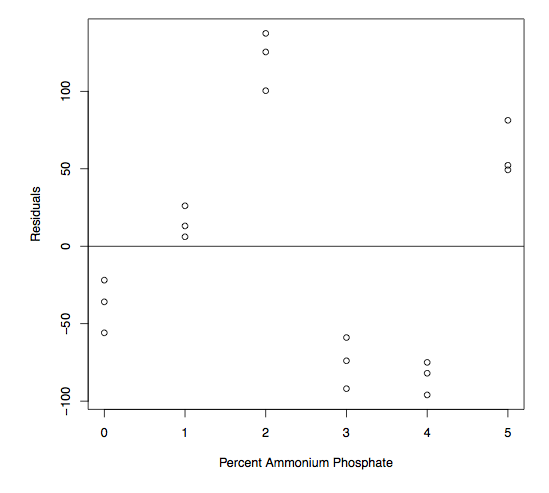
\includegraphics{../../fig/flyashquadres.png}
\end{frame}




\begin{frame}
\frametitle{Cubic fit: $\wh{y}_i = 1188 + 633 x - 214 x^22 + 18.3 x^3$}
\setkeys{Gin}{width=1\textwidth} 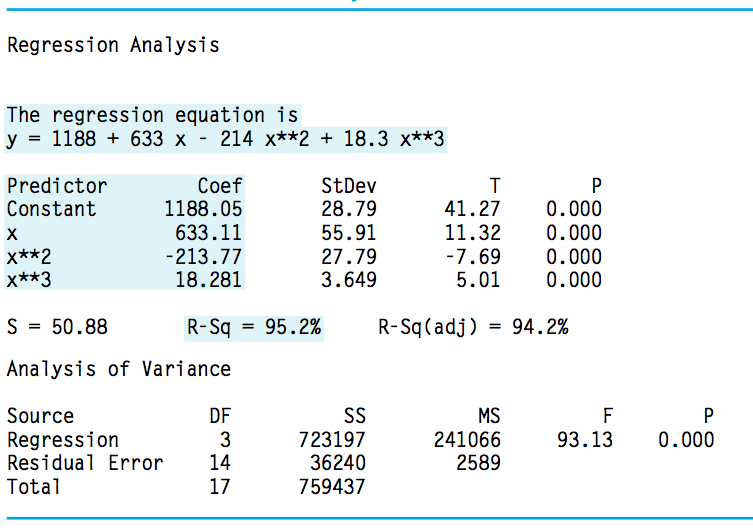
\includegraphics{../../fig/flyashcubicfitoutput.png}
\end{frame}

\begin{frame}
\frametitle{Cubic fit: $\wh{y}_i = 1188 + 633 x - 214 x^22 + 18.3 x^3$}
\setkeys{Gin}{width=.8\textwidth} 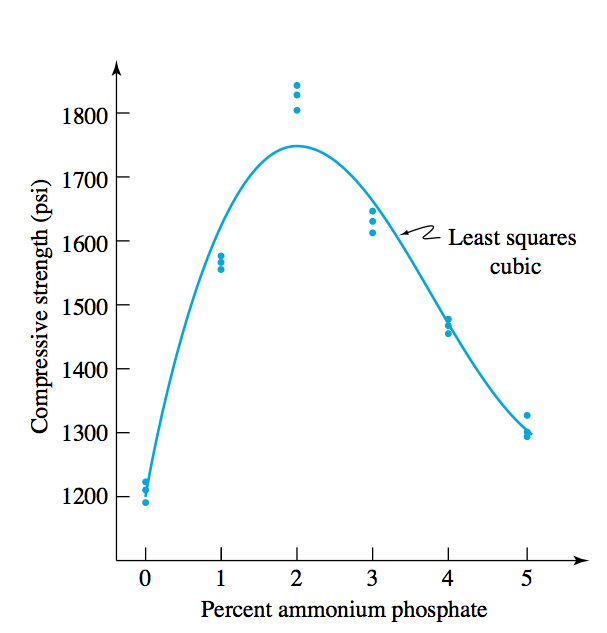
\includegraphics{../../fig/flyashcubicfitfit.png}
\end{frame}

\begin{frame}
\frametitle{$R^2$ rose to 95.2\%, and the residual plot improved.}
\setkeys{Gin}{width=.9\textwidth} 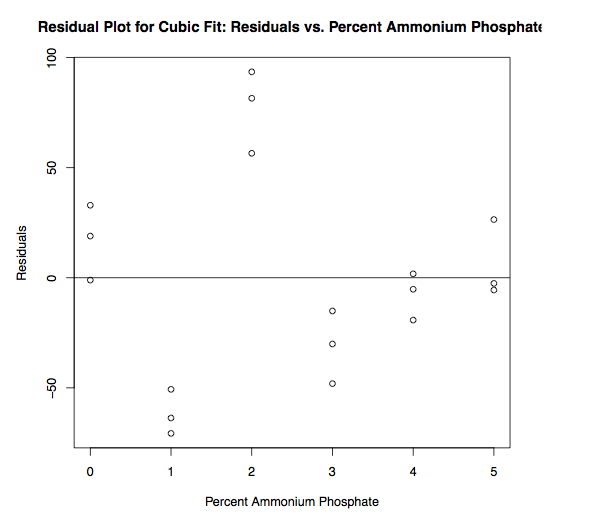
\includegraphics{../../fig/flyashcubicfitres.png}
\end{frame}





\section{Multiple Regression}

\begin{frame}
\frametitle{Multiple Regression}
\begin{itemize}
\pause \item {\bf Multiple Regression}: regression on multiple variables:
\pause \begin{align*}
y_i \approx b_0 + b_1 x_{i, 1} + b_2 x_{i, 2} + b_3 x_{i,3} + \cdots + b_{p-1} x_{i, {p-1}}
\end{align*}
\begin{itemize}
\pause \item The $p$ coefficients $b_0, b_1, \ldots, b_{p-1}$ are estimated by minimizing the loss function below using the least squares principle:
\pause \begin{align*} \scriptsize
S(b_0, \ldots, b_p) = \sum_{i = 1}^n (y_i -  (b_0 + b_1 x_{i, 1} + \cdots + b_{p-1} x_{i,p-1}))^2
\end{align*}
\pause \item In practice, we make a computer find the coefficients for us. This class uses JMP.
\end{itemize}
\end{itemize}
\end{frame}


\begin{frame}
\frametitle{Example: New York rivers data}
\begin{itemize}
\item Nitrogen content is a measure of river pollution. 
\end{itemize}
\setkeys{Gin}{width=1\textwidth} 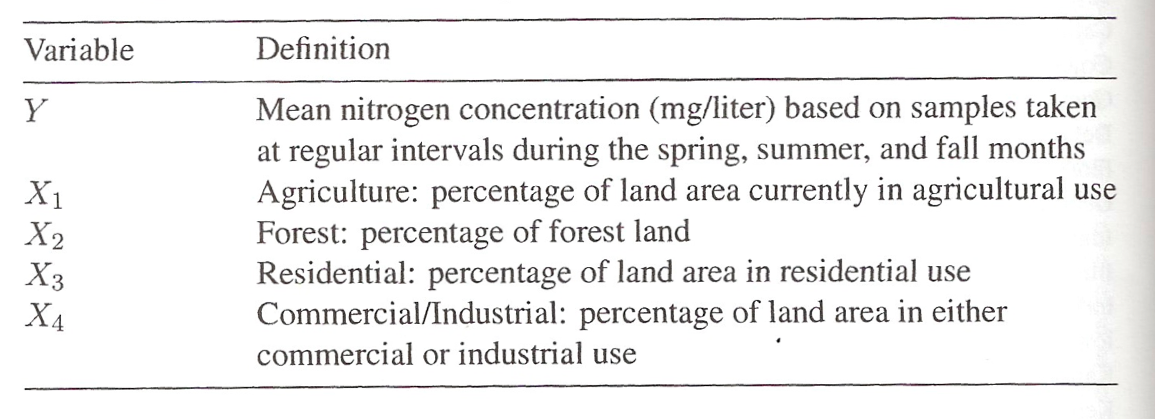
\includegraphics{../../fig/riversdefs.png}
\begin{itemize}
\pause \item I will fit each of:
\begin{align*}
\uncover<2->{\wh{y}_i} & \uncover<2->{= b_0 + b_1 x_{i, 1}} \\
\uncover<3->{\wh{y}_i }& \uncover<3->{= b_0 + b_1 x_{i, 1} + b_2 x_{i, 2}+ b_3 x_{i, 3}+ b_4 x_{i, 4}}
\end{align*}
\pause \pause and evaluate fit quality.
\end{itemize}
\end{frame}

\begin{frame}
\frametitle{Example: New York rivers data}
\setkeys{Gin}{width=1\textwidth} 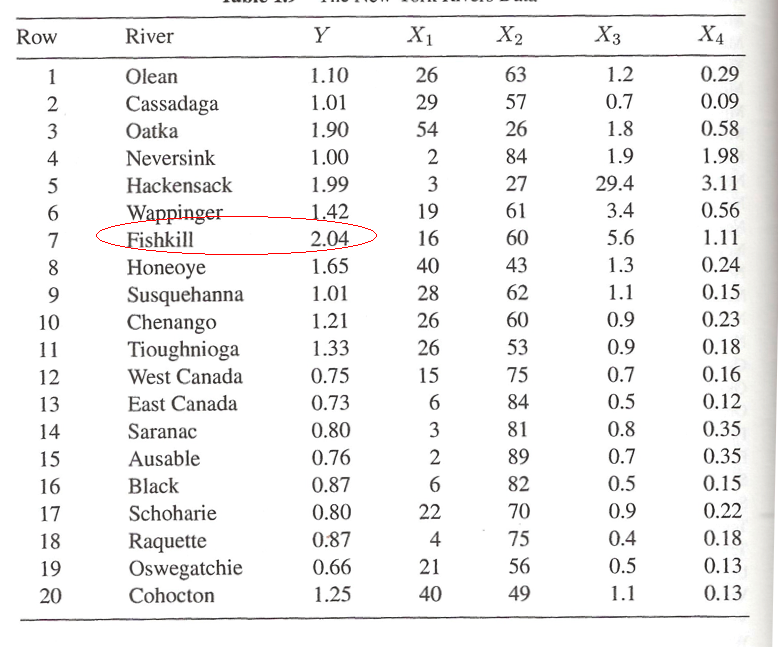
\includegraphics{../../fig/riversdata.png}
\end{frame}


\begin{frame}
\frametitle{$\wh{y}_i = b_0 + b_1 x_{i, 1} $: pollution vs. agricultural land.}
\begin{center}
\setkeys{Gin}{width=1\textwidth} 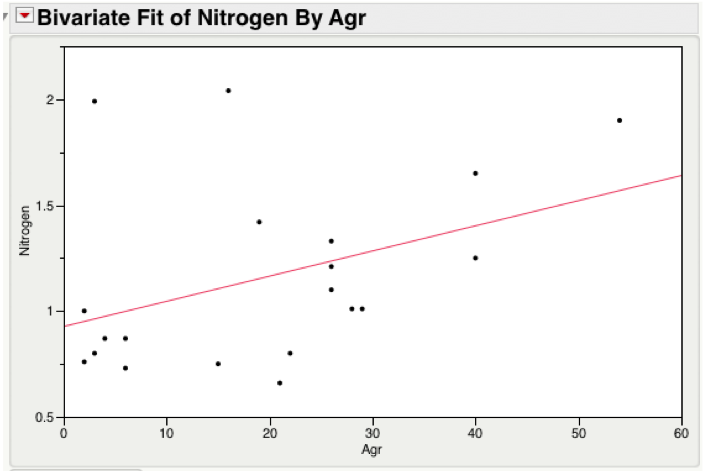
\includegraphics{../../fig/riversmodel1plot.png}
\end{center}
\begin{itemize}
\pause \item It looks like the data could be roughly linear, although there are too few points to be sure.
\end{itemize}
\end{frame}


\begin{frame}
\frametitle{$\wh{y}_i = b_0 + b_1 x_{i, 1} $: pollution vs. agricultural land.}
\begin{center}
\setkeys{Gin}{width=.75\textwidth} 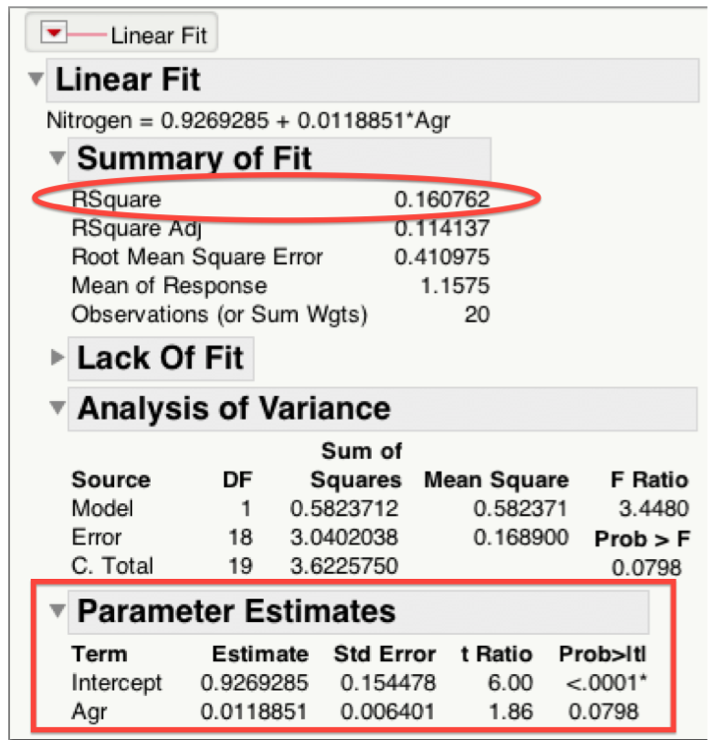
\includegraphics{../../fig/riversmodel1output.png}
\end{center}
\end{frame}


\begin{frame}
\frametitle{$\wh{y}_i = b_0 + b_1 x_{i, 1} $: pollution vs. agricultural land.}
\begin{center}
\setkeys{Gin}{width=1\textwidth} 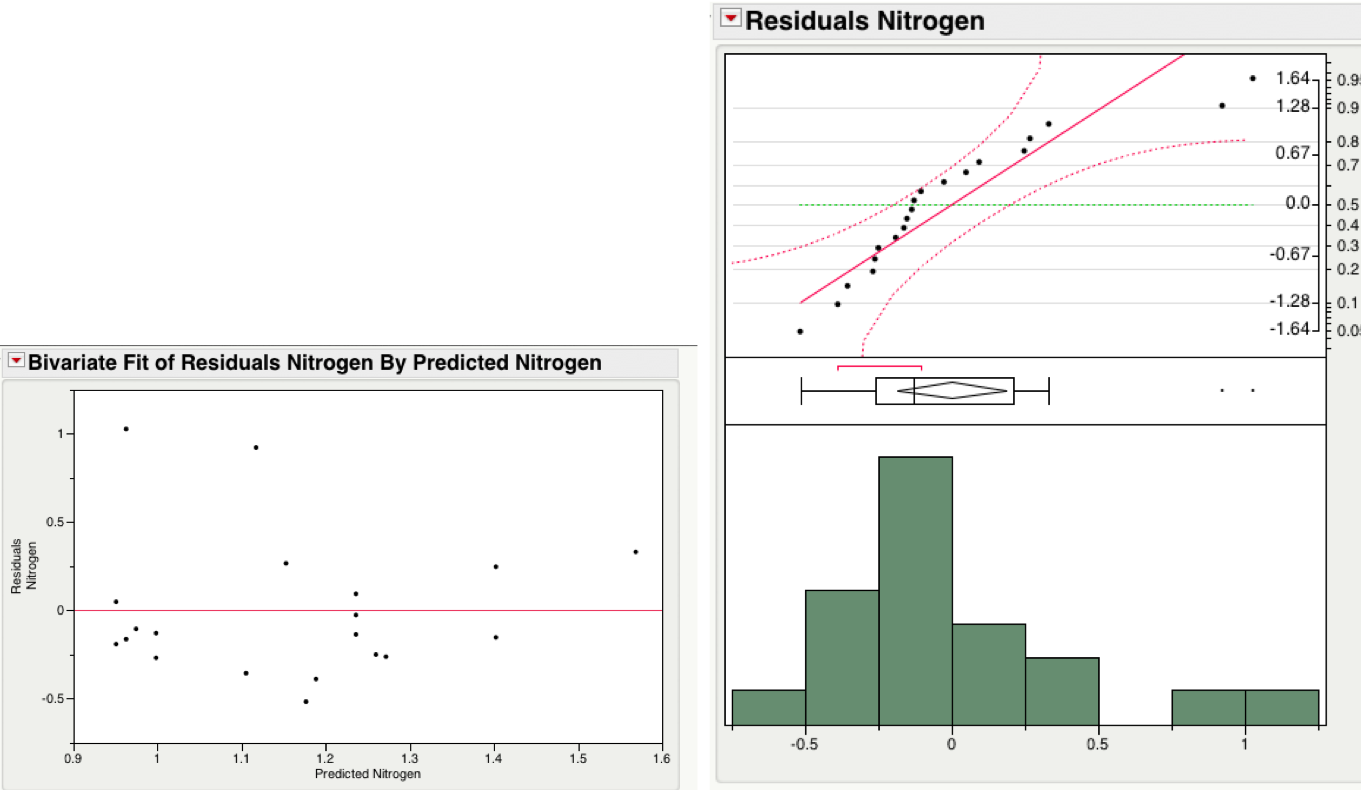
\includegraphics{../../fig/riversmodel1diagnostics.png}
\end{center}
\end{frame}

\begin{frame}
\frametitle{Conclusions: $\wh{y}_i = b_0 + b_1 x_{i, 1} $}
\begin{itemize}
\pause \item A low $R^2$ means the model isn't very useful for predicting the pollution of other New York rivers outside our dataset.
\pause \item However, the lack of a pattern in the residual plot shows that the model is valid.
\pause \item The residuals depart from a bell shape slightly, but not enough to interfere with statistical inference.
\end{itemize}
\end{frame}


\begin{frame}
\frametitle{$\wh{y}_i = b_0 + b_1 x_{i, 1}  + b_2 x_{i, 2} + b_3 x_{i, 3} + b_4 x_{i, 4}  $}
\setkeys{Gin}{width=.75\textwidth} 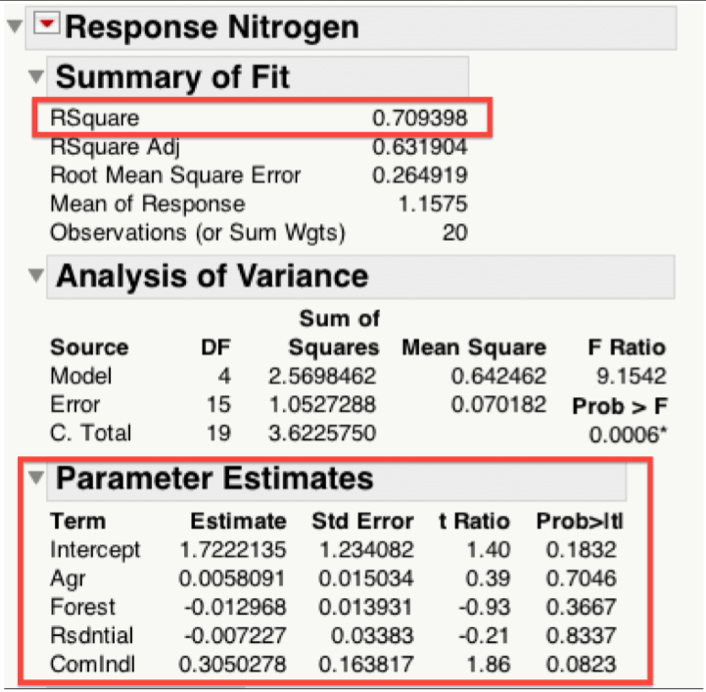
\includegraphics{../../fig/riversfullmodeloutput.png}

\end{frame}

\begin{frame}
\frametitle{Full model: observed pollution values vs fitted values}
\setkeys{Gin}{width=1\textwidth} 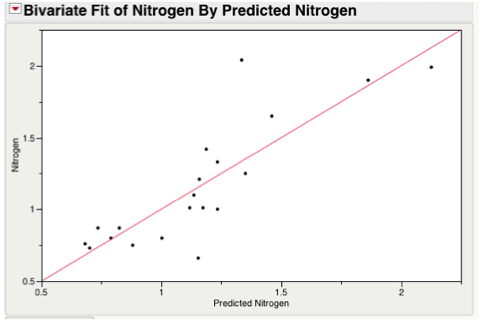
\includegraphics{../../fig/riversfullmodelrealvsfit.png}
\end{frame}


\begin{frame}
\frametitle{Full model: residual plots}
\setkeys{Gin}{width=1\textwidth} 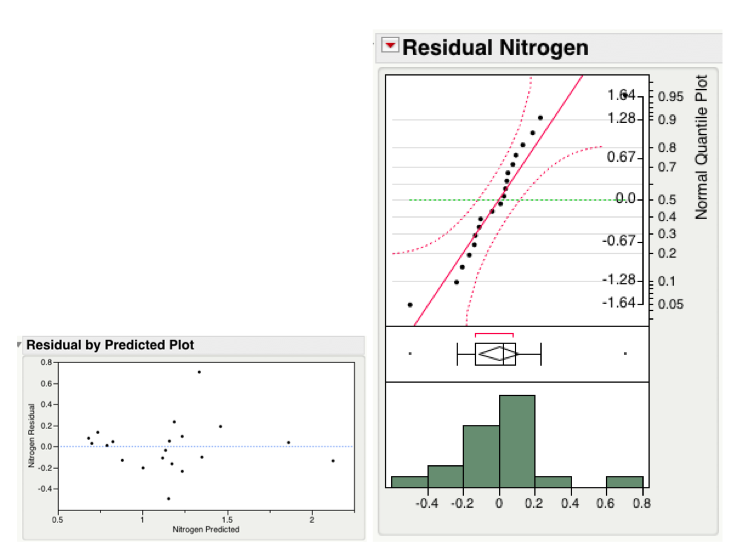
\includegraphics{../../fig/riversfullmodeldiag.png}
\end{frame}

\begin{frame}
\frametitle{Conclusions: full model}
\begin{itemize}
\pause \item A higher $R^2$ indicates that the full model is more useful for predicting river pollution than the agriculture-only model.
\pause \item The residual plots show that the full model is valid too.
\end{itemize}
\end{frame}

\begin{frame}
\frametitle{An even bigger model} \small  
\begin{itemize}
\pause \item From the scatterplot of $y$ on $x_4$, it looks like $x_4$ needs at least a quadratic term.
\begin{center}
\setkeys{Gin}{width=.4\textwidth} 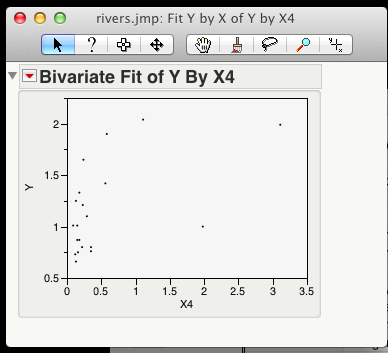
\includegraphics{../../fig/x41.png}
\end{center}
\pause \item I can fit the model:
\begin{align*}
\wh{y}_i = b_0 + b_1 x_{i, 1}  + b_2 x_{i, 2} + b_3 x_{i, 3} + b_4 x_{i, 4}  + c x_{i, 4}^2
\end{align*}
\pause which is a combination of polynomial regression and multiple regression.
\end{itemize}
\end{frame}

\begin{frame}
\frametitle{The JMP Spreadsheet}
\begin{center}
\setkeys{Gin}{width=1\textwidth} 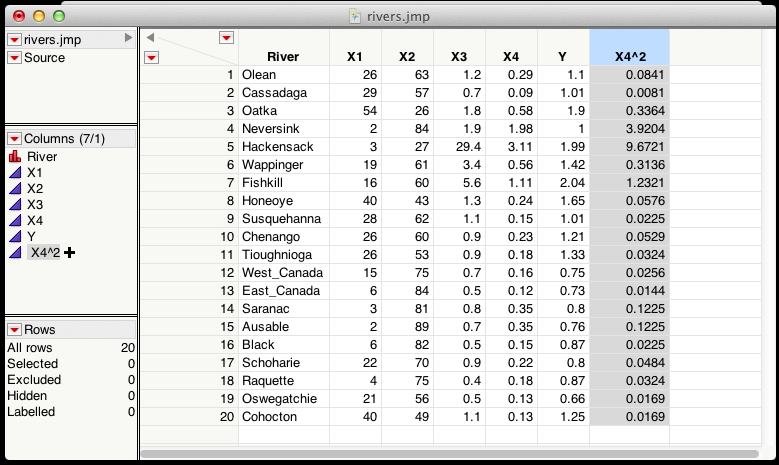
\includegraphics{../../fig/x42.png}
\end{center}
\end{frame}

\begin{frame}
\frametitle{$R^2$ improves}
\begin{center}
\setkeys{Gin}{width=.7\textwidth} 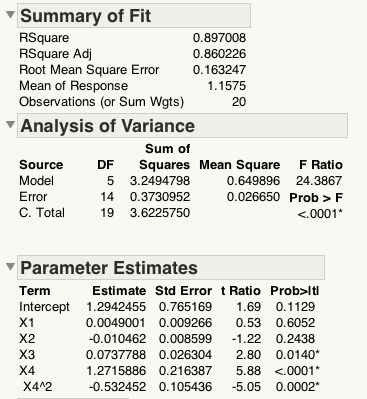
\includegraphics{../../fig/x43.png}
\end{center}
\end{frame}

\begin{frame}
\frametitle{The model looks valid: no pattern in the residuals}
\begin{center}
\setkeys{Gin}{width=1\textwidth} 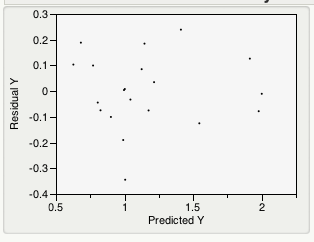
\includegraphics{../../fig/x44.png}
\end{center}
\end{frame}

\begin{frame}
\frametitle{\small The model can be used for statistical inference: the residuals look normally distributed.}
\begin{center}
\setkeys{Gin}{width=.6\textwidth} 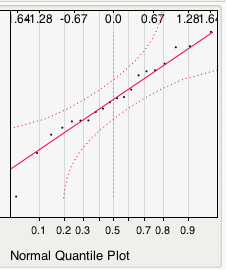
\includegraphics{../../fig/x45.png}
\end{center}
\end{frame}



\end{document}
